\subsection{Виды предметно-ориентированных языков программирования} \label{sub122}
Глобально предметно-ориентированные языки программирования делятся на~две~группы: 
\begin{itemize} 
	\item{внешние;}
	\item{внутренние.}
\end{itemize}

Разработка внешних языков состоит из~трёх этапов:

\begin{itemize} 
	\item{определение семантической модели;}
	\item{определение синтаксической модели (абстрактный и~конкретный синтаксис);}
	\item{определение правил трансформации (правила, по~которым абстрактное представление транслируется в~исполнимое).}
\end{itemize}

Для генерации лексического и~синтаксического анализатора внешних языков существуют готовые средства, например, связка программ Lex и Yacc, входящая в~стандарт POSIX. 

Достоинством внешних DSL является узкая специализация, что облегчает процесс решения предметных задач, а~также гибкая базовая грамматика. Но~у~внешних языков существует и~ряд недостатков. Например, среду разработки, которая поддерживает и~облегчает написание сценариев на~внешнем DSL, обычно разрабатывают либо с~нуля, либо как дополнение к~уже существующей современной интегрированной среде разработки(Integrated Development Environment, IDE). Также, наряду с~лёгкостью решения предметных задач, внешние DSL практически никогда не~подходят для решения задач в~смежных областях.

Альтернативой внешним DSL являются внутренние. Внутренний DSL (Embedded Language)~--- это подмножество других языков программирования широкого применения~\cite{VanDeursen2000}. Такой подход позволяет совместить выразительность и~мощь предметно-ориентированного языка вместе с~возможностями языков широкого применения (Haskell, Python, Groovy, Scala, Kotlin, Ruby, C\#, F\#). 

Выбирая современный язык программирования общего назначения как основу для создания внутреннего DSL, можно сразу получить готовый набор средств поддержки разработки~--- современные IDE, которые поддерживают базовый язык~\cite{Botov}. Подходы к созданию DSL, языки и инструментарий представлены на~рис.~\ref{img:dsl}.

\newpage

\begin{figure}[ht]
	\centering
	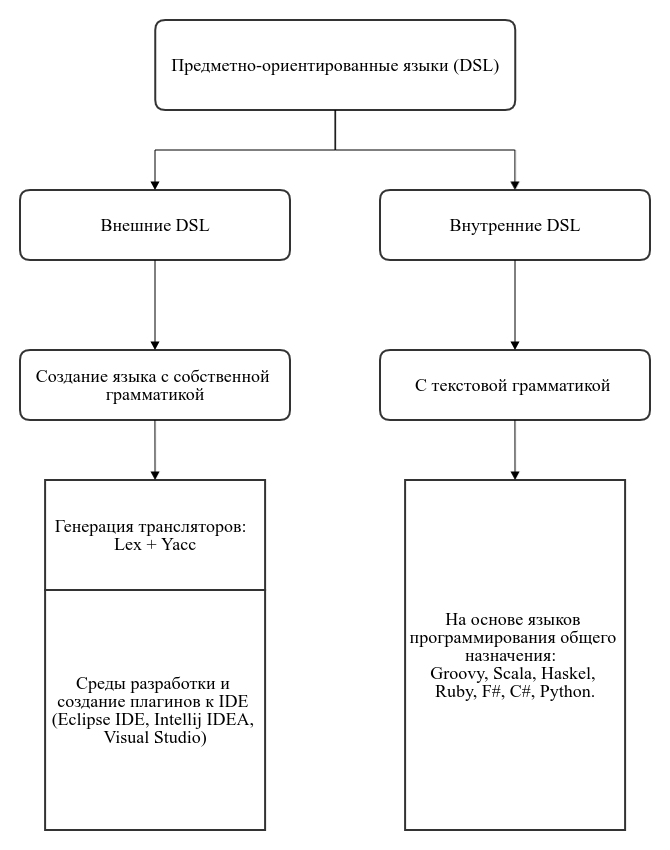
\includegraphics [scale=0.65] {dsl}
	\caption{Подходы к созданию внешних и внутренних DSL, \\ языки и~инструментарий
		создания и поддержки DSL}
	\label{img:dsl}
\end{figure}

При разработке внутренних DSL возникают ситуации, когда IDE не~может определить некоторые конструкции языка. Это может быть часть языка DSL, которая будет интерпретированна только во~время выполнения программы (Groovy DSL). Или допустимый домен атрибута (переменной) может зависеть от~окружения, в~котором находится содержащий его файл, что значительно усложняет статический анализ, производимый IDE.


